\section{独立样本的误差}
\label{sec:mcerr-iid}

最理想的情形是生成程序给出独立且精确服从$\pi$的样本$X_1,\dots,X_N$。这时偏差为零：由上一节，每个$X_i$都服从$\pi$，所以$\mathbb{E}[\hat{I}_N]=I$。$f(X_1),f(X_2),\dots$独立同分布且可积，由第~\ref{chap:laws-of-large-numbers}章的强大数律，
\begin{equation}
 \hat{I}_N\xrightarrow{\mathrm{a.s.}}I .
 \label{eq:mcerr-consistency}
\end{equation}
无偏说的是平均意义下没有系统偏离，一致性说的是几乎每一次计算都会随$N$增大而接近$I$。两者都不回答一个实际问题：给定的$N$下误差有多大，或者要达到给定精度需要多大的$N$。回答它需要比可积更多的信息，所需的矩条件也决定了能给出什么样的保证。

\subsection{有限样本误差界}
\label{sec:mcerr-finite-bound}

第一种保证对每个具体的$N$成立，代价是要求$f$的二阶矩有限。记$\sigma_f^{2}=\operatorname{Var}_{\pi}(f)$，即$f(X)$在$X\sim\pi$时的方差。

\begin{theorem}[独立样本平均的误差界]
\label{thm:mcerr-iid-bound}
设$X_1,\dots,X_N$独立且都服从$\pi$，$\mathbb{E}_{\pi}[f^{2}]<\infty$。则
\begin{equation}
 \operatorname{Var}(\hat{I}_N)=\frac{\sigma_f^{2}}{N},\qquad \sqrt{\mathbb{E}\bigl[(\hat{I}_N-I)^{2}\bigr]}=\frac{\sigma_f}{\sqrt{N}} ,
 \label{eq:mcerr-iid-var}
\end{equation}
并且对每个$\varepsilon>0$，
\begin{equation}
 \mathbb{P}\bigl(\lvert\hat{I}_N-I\rvert\geq\varepsilon\bigr)\leq\frac{\sigma_f^{2}}{N\varepsilon^{2}} .
 \label{eq:mcerr-chebyshev}
\end{equation}
\end{theorem}

\begin{proof}
独立随机变量和的方差等于方差之和，所以
\[
 \operatorname{Var}(\hat{I}_N)=\frac{1}{N^{2}}\sum_{i=1}^{N}\operatorname{Var}\bigl(f(X_i)\bigr)=\frac{N\sigma_f^{2}}{N^{2}}=\frac{\sigma_f^{2}}{N} .
\]
偏差为零，由定理~\ref{thm:mcerr-mse}，均方误差等于这个方差，开方得到均方根误差。对$\hat{I}_N$用第~\ref{chap:tail-probabilities}章的Chebyshev不等式，就得到式~\eqref{eq:mcerr-chebyshev}。
\end{proof}

式~\eqref{eq:mcerr-iid-var}是Monte Carlo方法最重要的一个公式。误差按$N^{-1/2}$缩小，与$\mathcal{X}$的维数没有直接关系；维数只通过$\sigma_f$间接进入。精度提高到十倍，样本数要增加到一百倍。反过来解式~\eqref{eq:mcerr-chebyshev}：要使误差超过$\varepsilon$的概率不超过$\delta$，只需
\begin{equation}
 N\geq\frac{\sigma_f^{2}}{\delta\varepsilon^{2}} .
 \label{eq:mcerr-sample-size}
\end{equation}

\paragraph{算一个具体的样本量}
对$f(u)=\mathrm{e}^{u}$，$\pi=\operatorname{Unif}(0,1)$，先求二阶矩
\[
 \mathbb{E}[\mathrm{e}^{2U}]=\int_0^1\mathrm{e}^{2u}\,\mathrm{d}u=\frac{\mathrm{e}^{2}-1}{2}=3.1945 .
\]
再减去$I^{2}=(\mathrm{e}-1)^{2}=2.9525$，得到
\[
 \sigma_f^{2}=3.1945-2.9525=0.2420,\qquad \sigma_f=0.4920 .
\]
$N=100$时均方根误差为$0.0492$，$N=10^{4}$时为$0.00492$。图~\ref{fig:mcerr-rmse-rate}(a)把每个$N$下$1000$次独立重复得到的均方根误差与$\sigma_f/\sqrt{N}$画在双对数坐标中，点落在斜率为$-1/2$的直线上。

取$\varepsilon=0.01$，$\delta=0.05$，式~\eqref{eq:mcerr-sample-size}给出
\[
 N\geq\frac{0.2420}{0.05\times10^{-4}}=48407.1 ,
\]
即$N=48408$足够。图~\ref{fig:mcerr-chebyshev}比较了这个上界与实际概率。实际概率在$N=10^{4}$时已经降到约$0.044$；下一小节的正态近似给出所需样本量约$9298$。Chebyshev界保守了大约五倍，但它对每个$N$、对所有方差为$0.2420$的被积函数都成立，不需要任何极限论证。若$f$有界，第~\ref{chap:tail-probabilities}章的指数矩方法还能把对$\delta$的依赖从$1/\delta$改进为$\ln(1/\delta)$。

\begin{BookInlineFigure}
 \centering
 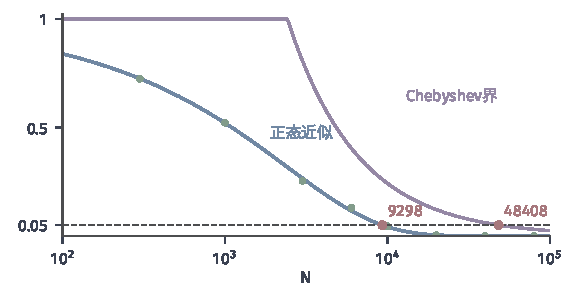
\includegraphics[width=96mm]{figures/07-probability/08-sampling-and-integration/matplotlib/mcerr-chebyshev/figure.pdf}
 \caption{$f(u)=\mathrm{e}^{u}$的样本平均误差至少为$\varepsilon=0.01$的概率。紫线为Chebyshev界$\min\{1,\sigma_f^{2}/(N\varepsilon^{2})\}$，蓝线为正态近似$2(1-\Phi(\varepsilon\sqrt{N}/\sigma_f))$，绿点为每个$N$下$2000$次重复的频率（种子$3104$）。红点标出两条曲线降到$0.05$时的样本量。}
 \label{fig:mcerr-chebyshev}
\end{BookInlineFigure}

\paragraph{二阶矩不可省}
$N^{-1/2}$的尺度完全来自方差有限。只有$\mathbb{E}_{\pi}\lvert f\rvert<\infty$时，式~\eqref{eq:mcerr-consistency}仍然成立，但误差缩小的速度可以慢得多。取$f(u)=u^{-3/4}$，$\pi=\operatorname{Unif}(0,1)$，则
\[
 I=\int_0^1u^{-3/4}\,\mathrm{d}u=4,\qquad \mathbb{E}[f(U)^{2}]=\int_0^1u^{-3/2}\,\mathrm{d}u=\infty .
\]
$f$在$0$附近趋于无穷，偶尔抽到很小的$u$，就产生一个很大的函数值。

这些大值决定了误差的尺度。$f(U)>t$当且仅当$U<t^{-4/3}$，所以
\[
 \mathbb{P}\bigl(f(U)>t\bigr)=t^{-4/3},\qquad t\geq1 .
\]
$N$个样本中至少有一个超过$t$的概率约为$Nt^{-4/3}$，它在$t\approx N^{3/4}$时变为一的量级。于是$N$个样本中最大的函数值通常在$N^{3/4}$附近，它对平均的贡献约为$N^{3/4}/N=N^{-1/4}$。每个尺度上都以不可忽略的概率出现这样的大项，平均的误差也就按$N^{-1/4}$而不是$N^{-1/2}$缩小。把这个论证写严格，需要独立和在无穷方差下的极限理论，篇幅较长，读者可查阅~\scite{math-kallenberg2021probability}。

图~\ref{fig:mcerr-heavy-paths}(a)是五次运行的运行平均：路径大部分时间偏低，每遇到一个很小的$u$就向上跳一次，然后慢慢回落。图(b)画出最大单项对平均的贡献$\max_{i\leq N}f(U_i)/N$，它沿着$N^{-1/4}$下降。图~\ref{fig:mcerr-rmse-rate}(b)用中位绝对误差衡量精度（均方误差在这里是无穷），它从$N=100$时的$0.986$降到$N=10^{5}$时的$0.172$，比值$5.73$与$1000^{1/4}=5.62$相符。按这个速度，误差缩小到十分之一要把样本数增加一万倍。

\begin{BookInlineFigure}
 \centering
 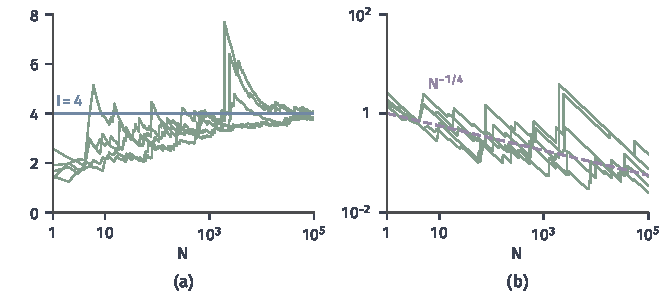
\includegraphics[width=112mm]{figures/07-probability/08-sampling-and-integration/matplotlib/mcerr-heavy-paths/figure.pdf}
 \caption{$f(u)=u^{-3/4}$的五次独立运行（种子$3105$至$3109$），横轴为对数刻度。(a)运行平均（绿线）与$I=4$（蓝线）；(b)最大单项的贡献$\max_{i\leq N}f(U_i)/N$（绿线）与参考线$N^{-1/4}$（紫色虚线），纵轴为对数刻度。}
 \label{fig:mcerr-heavy-paths}
\end{BookInlineFigure}

\begin{BookInlineFigure}
 \centering
 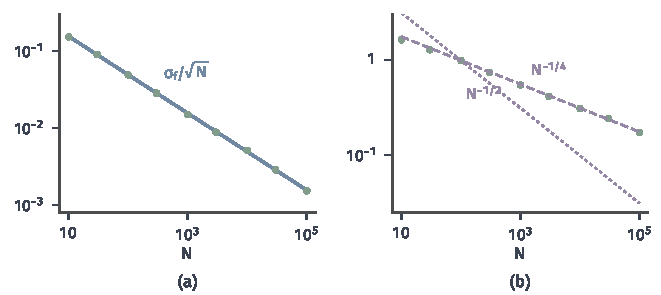
\includegraphics[width=112mm]{figures/07-probability/08-sampling-and-integration/matplotlib/mcerr-rmse-rate/figure.pdf}
 \caption{误差随样本数的变化，双对数坐标，每个$N$重复$1000$次。(a)$f(u)=\mathrm{e}^{u}$：绿点为模拟的均方根误差（种子$3102$），蓝线为$\sigma_f/\sqrt{N}$；(b)$f(u)=u^{-3/4}$：绿点为中位绝对误差（种子$3103$），紫色虚线与点线分别是斜率$-1/4$与$-1/2$的参考线。}
 \label{fig:mcerr-rmse-rate}
\end{BookInlineFigure}

\subsection{渐近误差区间}
\label{sec:mcerr-asymptotic-interval}

Chebyshev界保守，因为它只用了方差。样本数较大时，中心极限定理给出误差的近似分布，从而给出更紧的误差范围。实际计算中$\sigma_f$通常未知，要用同一批样本估计它。样本函数值的样本方差记为
\begin{equation}
 S_N^{2}=\frac{1}{N-1}\sum_{i=1}^{N}\bigl(f(X_i)-\hat{I}_N\bigr)^{2},\qquad N\geq2 .
 \label{eq:mcerr-sample-var}
\end{equation}

\begin{theorem}[独立样本的渐近误差区间]
\label{thm:mcerr-iid-clt}
设$X_1,X_2,\dots$独立且都服从$\pi$，$0<\sigma_f^{2}<\infty$。则
\begin{equation}
 \frac{\sqrt{N}\,(\hat{I}_N-I)}{S_N}\xrightarrow{\mathrm{d}}\mathcal{N}(0,1) .
 \label{eq:mcerr-studentized}
\end{equation}
因此对$0<\alpha<1$及$z=\Phi^{-1}(1-\alpha/2)$，
\begin{equation}
 \lim_{N\to\infty}\mathbb{P}\Bigl(I\in\Bigl[\hat{I}_N-\frac{zS_N}{\sqrt{N}},\ \hat{I}_N+\frac{zS_N}{\sqrt{N}}\Bigr]\Bigr)=1-\alpha .
 \label{eq:mcerr-iid-interval}
\end{equation}
\end{theorem}

\begin{proof}
$f(X_i)$独立同分布，方差为有限正数$\sigma_f^{2}$。由第~\ref{chap:central-limit-theorem}章独立同分布的中心极限定理，
\[
 \frac{\sqrt{N}\,(\hat{I}_N-I)}{\sigma_f}\xrightarrow{\mathrm{d}}\mathcal{N}(0,1) .
\]
由第~\ref{chap:laws-of-large-numbers}章样本方差的强大数律，$S_N^{2}\to\sigma_f^{2}$几乎必然成立，因而$\sigma_f/S_N\to1$依概率成立（$S_N=0$的概率趋于零，在该事件上任意规定比值即可）。式~\eqref{eq:mcerr-studentized}的左边是上式左边乘以$\sigma_f/S_N$，由第~\ref{chap:weak-convergence-of-distributions}章的Slutsky定理，乘积依分布收敛到$\mathcal{N}(0,1)$。

标准正态分布函数连续，由同一章的分布函数判据，对每个$z$，
\[
 \mathbb{P}\Bigl(\Bigl\lvert\frac{\sqrt{N}(\hat{I}_N-I)}{S_N}\Bigr\rvert\leq z\Bigr)\to\Phi(z)-\Phi(-z)=1-\alpha .
\]
左边的事件正是$I$落在式~\eqref{eq:mcerr-iid-interval}的区间中。
\end{proof}

式~\eqref{eq:mcerr-iid-interval}中的区间称为\term{渐近误差区间}（asymptotic error interval），$1-\alpha$称为名义覆盖概率；$\alpha=0.05$时$z=1.96$。区间宽度与$S_N/\sqrt{N}$成正比，后者称为估计的标准误差。它与Chebyshev界的区别在于保证的类型：Chebyshev界对每个$N$成立但偏松，渐近区间只在$N\to\infty$时给出正确的覆盖概率，对固定的$N$没有任何保证。若$\sigma_f$已知且三阶矩有限，第~\ref{chap:central-limit-theorem}章的Berry--Esseen界给出正态近似误差按$N^{-1/2}$缩小的上界；改用$S_N$以后还要加上方差估计的误差。

\paragraph{五个点的区间}
用上一节的五个均匀随机数。函数值的平均为$1.8233$，由式~\eqref{eq:mcerr-sample-var}，
\[
 S_5^{2}=0.3391,\qquad S_5=0.5823 .
\]
$\alpha=0.05$时区间半宽为
\[
 \frac{1.96\times0.5823}{\sqrt5}=0.5104 ,
\]
区间为$[1.3129,\,2.3337]$，包含$I=1.7183$。但这一次包含不说明区间可靠。图~\ref{fig:mcerr-rare-coverage}(b)的蓝线是每个$N$下$20000$次重复的实际覆盖频率：$N=5$时只有$0.868$，$N=20$时为$0.935$，$N\geq100$以后才与$0.95$相差无几。

\paragraph{稀有的大贡献}
覆盖概率接近名义值所需的样本数可以大得多。设$\pi=\operatorname{Unif}(0,1)$，
\[
 f(u)=1+1000\cdot\mathbf{1}_{\{u>0.999\}} .
\]
它有界，各阶矩都有限，定理~\ref{thm:mcerr-iid-clt}的条件全部满足。积分与方差分别是
\[
 I=1+1000\times0.001=2,\qquad \sigma_f^{2}=1000^{2}\times0.001\times0.999=999 .
\]
积分的一半来自一个概率只有千分之一的区域。

取$N=500$。一次也没有抽到$u>0.999$的概率是
\[
 0.999^{500}=\mathrm{e}^{500\ln0.999}=0.6064 .
\]
在这个事件上，所有函数值都等于$1$，于是$\hat{I}_N=1$，$S_N=0$，区间退化为单点$\{1\}$，不包含$I=2$。计算者看到的是一组完全一致的函数值和零标准误差，没有任何迹象显示有问题。

若恰好抽到一次，$\hat{I}_N=1+1000/500=3$。$499$个值与平均相差$-2$，一个值相差$998$，所以
\[
 S_N^{2}=\frac{499\times4+998^{2}}{499}=\frac{998000}{499}=2000 ,
\]
区间半宽为$1.96\sqrt{2000/500}=3.92$，区间$[-0.92,\,6.92]$包含$2$。把抽中次数服从$\operatorname{Bin}(500,0.001)$的各种情形逐一相加，$N=500$时的实际覆盖概率只有$0.393$。

图~\ref{fig:mcerr-rare-coverage}(b)的黄线是这个覆盖概率随$N$的变化，按二项分布精确求和得到。$N=10^{3}$时为$0.632$，$N=10^{4}$时才到$0.926$。图(a)是五次运行的运行平均：每条路径都先平稳地停在$1$，直到第一次抽中才突然跳起。在跳起之前，运行平均、样本方差和区间都“看起来稳定”。

即使把同一计算独立重复五次，五次都没有抽中的概率仍有$0.6064^{5}=0.082$。重复运行可以发现运行之间的分歧，但发现不了每次运行都漏掉的东西。定理~\ref{thm:mcerr-iid-clt}在这里并没有失效，它只说$N$足够大时覆盖概率接近名义值；“足够大”要比$1/0.001$大很多，而这个尺度是由$f$的结构决定的，从样本中看不出来。能防止这类错误的，是对$f$与$\pi$本身的分析，例如知道函数值的上界或贡献集中的区域，第~\ref{chap:variance-reduction}章的重要性采样正是利用这类信息。

\begin{BookInlineFigure}
 \centering
 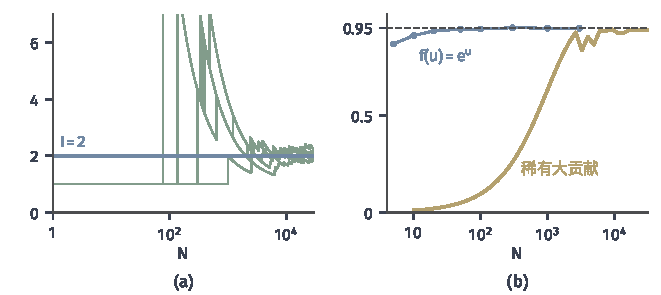
\includegraphics[width=112mm]{figures/07-probability/08-sampling-and-integration/matplotlib/mcerr-rare-coverage/figure.pdf}
 \caption{稀有大贡献$f(u)=1+1000\cdot\mathbf{1}_{\{u>0.999\}}$，$I=2$。(a)五次独立运行的运行平均（绿线，种子$3110$至$3114$）与$I$（蓝线），横轴为对数刻度；(b)渐近区间$\hat{I}_N\pm1.96S_N/\sqrt{N}$的实际覆盖概率：黄线为稀有大贡献的精确值，蓝线为$f(u)=\mathrm{e}^{u}$在每个$N$下$20000$次重复的频率（种子$3115$），虚线为名义值$0.95$。}
 \label{fig:mcerr-rare-coverage}
\end{BookInlineFigure}
